\documentclass[12pt,onesided,fullpage]{amsart}

%%% PAGE DIMENSIONS
\usepackage{multirow}
\usepackage{placeins}
\usepackage[top=1in, bottom=1in, left=1in, right=1in]{geometry}
%\pdfpagewidth=8.5in % for pdflatex
%\pdfpageheight=11in % for pdflatex

\usepackage{graphicx} % support the \includegraphics command and options

%%% PACKAGES
\usepackage{booktabs} % for much better looking tables
\usepackage{array} % for better arrays (eg matrices) in maths
\usepackage{paralist} % very flexible & customisable lists (eg. enumerate/itemize, etc.)
\usepackage{verbatim} % adds environment for commenting out blocks of text & for better verbatim

%%% HEADERS & FOOTERS
\usepackage{fancyhdr} % This should be set AFTER setting up the page geometry
\pagestyle{fancy} % options: empty , plain , fancy
\renewcommand{\headrulewidth}{0pt} % customise the layout...

\usepackage{amsfonts}
\usepackage{amsmath}
\usepackage{amssymb}
\usepackage{array,amsmath,graphicx,psfrag,amssymb,subfigure,tabularx,booktabs}
\usepackage{mparhack}
\usepackage{setspace}
\usepackage{natbib}
\usepackage{multicol}
\usepackage{color}
\usepackage{dcolumn}
\usepackage{hyperref}
\usepackage{stmaryrd}
\usepackage{placeins}
\setcitestyle{authordate,round,semicolon,aysep={,},yysep={,}}
\bibpunct[:]{(}{)}{;}{a}{,}{,}

% \doublespacing
\def\input@path{
	{C:/Users/Owner/Research/netsMatter/paper/graphics/},
	{C:/Users/herme/Research/netsMatter/paper/graphics/},
	{/Users/s7m/Research/netsMatter/paper/graphics/},
	{/Users/dorffc/ProjectsGit/netsMatter/paper/graphics}
}

\graphicspath{
	{C:/Users/Owner/Research/netsMatter/paper/graphics/},
	{C:/Users/herme/Research/netsMatter/paper/graphics/},
	{/Users/s7m/Research/netsMatter/paper/graphics/},
	{/Users/dorffc/ProjectsGit/netsMatter/paper/graphics}
}

\begin{document}
\singlespacing

\title[PSRM-OA-2019-0126]{Ms. No. PSRM-OA-2019-0126 entitled ``Taking Dyads Seriously''}

\date{\today~~Version 0.01}
\maketitle

$\hspace{-5mm}$Dear Editors, \\ [1ex]

Thank you for the opportunity to revise and resubmit our manuscript. We believe the manuscript has benefited from the Reviewers' helpful and thoughtful comments. We have revised the manuscript, taking seriously each individual point raised by the Reviewers. Our comments and responses are shown in \textcolor{blue}{\emph{BLUE}} below each of the points made by the Reviewers.

We hope you agree that the manuscript has improved through this process and we are looking forward to your response.\\ [1ex]

% Sincerely, \\ [1ex]

% The Authors

\section*{Reviewer 1}

\begin{enumerate}
	\item P1: ``Most standard approaches assume that the problems raised by non-iid relational data can be addressed by recalculating the standard errors of estimated parameters to reflect the potential clustering of cases. In practice, such strategies rarely work because they do not directly address the fundamental data generating process.'' The term “rarely work” is too casual.  What problem exactly is motivating this paper?  E.g., the Aronow et al. paper cited at the start of the same paragraph looks at consistent variance estimators for semiparametric regression estimators on dyadic data. By the standards set out by those authors in that paper, the strategies “work” just fine.  I suppose then that the current paper has a different sense of what it means for something “to work.” For example, I am supposing that the current paper is talking about people misconstruing the structural interpretation of a reduced form parameter estimated in a GLM fit to dyadic data.  That would be wholly orthogonal to what Aronow et al. were considering, but then this needs explication.
	\begin{itemize}
		\item \textcolor{blue}{ \emph{
		We thank the reviewer for taking the time to provide these valuable comments. We have clarified our language in the paper to address this question.  Strategies like those employed by Aronow et al. do not directly model all relevant dependencies in the data but instead adjust the variance estimator. As Aronow et al. explain, ``Of course, accounting for dynamic dyadic clustering may fail to fully account for all relevant dependencies in the data'' (p. 16).   While such an approach decreases the risk of a type 1 error, it increases risk of type 2 error (if the mean estimate is biased downwards, increasing the variance estimate will lead us to falsely accept the null). The main aims of our research are to account for the relevant dependency structures in the data thereby enabling more accurate inference for covariates and to enable applied scholars using this framework to understand how to better understand the types of dependencies that exist in their data.
		}}
	\end{itemize}
	\item P2: “Scholars working with dyadic data typically begin by stacking observations associated with each dyad on top of one another. This makes sense if each observation is independent of the others.” Revise this opening, since it is perfectly fine to stack observations and then incorporate auxiliary information (such as adjacency matrix) to characterize dependencies between rows.
	\begin{itemize}
		\item \textcolor{blue}{ \emph{
		 The point is well taken, we have clarified this section (on page 2) to point to the assumption of independence as the primary problem, not the stacking of observations in and of itself.
		}}
	\end{itemize}
	\item P3: “Unless one is able to develop a model that can account for the variety of explanations that may play a role in determining why a particular actor is more active than others, parameter estimates from standard statistical models will be biased.” This is another example of language that is too causal and imprecise, like the opening paragraph. What are “parameter estimates from standard statistical models”?  And “biased” with respect to what target of inference? Again, I think the authors have in mind “bias” with respect to parameters that are meant to have a particular structural interpretation, but this needs to be clarified. Generally, section 2 should be clearer in motivating the problem.  Provide us with a toy example that illustrates the kind of “bias” that the paper has in mind from “standard models”.  For me at least, after reading section 2 I still wasn’t sure what problem the paper is actually trying to address.
	\begin{itemize}
		\item \textcolor{blue}{ \emph{
		We thank the reviewer for this suggestion. We have thoroughly revised the beginning of section two, so that the paper is clearer on the problem that it is seeking out.
	}}
	\end{itemize}
	\item P7: Regarding the specification, this augments a dyadic random effects model, which is quite common, with  the LFM component, which resembles an interactive fixed effects specification (cf. Bai 2009, Ecta) and is based on an SVD factorization of the observed network. It is useful to think of the infeasible estimator and the implications for interpreting the LFM component.  The infeasible estimator takes the transformation f(.), fixed effects parameters, and SRRM random effects as known, in which case the LFM amounts to predictions from a factor model fit to the adjacency matrix of residuals on the scale of the latent outcome.  Would this be a reasonable interpretation? If so it would be useful to draw the connection to factor models commonly in use these days (such as the interactive fixed effects model of Bai, which is the basis of, e.g., generalized synthetic control methods).
	\begin{itemize}
		\item \textcolor{blue}{ \emph{
		We thank the reviewer for providing this reference and have added discussion of Bai's work on interactive fixed effects to the manuscript. Within both Bai's work and the model we discuss here the goal is to find ways to use latent factor approaches to model heterogeneity. We'd also note that the recommender system literature from computer science also has its roots in using latent factor models to find low rank approximations. We had noted that already in the manuscript but have tried to make the link clearer in the revised ``Additive and Multiplicative Effect Models for Networks'' section.
		}}
	\end{itemize}
	\item P8: “accounting for this structure is necessary if we are to adequately represent the data generating process.” Continuing with the problems I have with the language above, what does “adequately represent” mean?. P9: “a) biased estimates of the effect of independent variables, b) uncalibrated confidence intervals, and c) poor predictive performance.” Okay here is where the paper are starting to clarify goals.  So a) is about causal identification.  But as I understand, the solution here is parametric identification of causal effects.  This means that the issue of misspecification and robustness ought to be taken up.  Similarly, b) is addressed in this paper under a fairly simple parametric data generating process. But again, how robust is the proposed model to situations where the real DGP does not abide by the parametric assumptions (linearity, normally distributed random effects, and a factor model for the residuals of dimension K)? For c), I think most would agree that the “proof” is simply in comparison to whatever other good models are available.  Not however, that in social science applications, forecasting and therefore c) are rarely of interest (at least not in the types of research that appear in political science journals).  As such, from the perspective of what the researchers in discipline mostly cares about, a) and b) are of primary importance.
	\begin{itemize}
		\item \textcolor{blue}{ \emph{
			For part (a), we have clarified that our study does not address causal identification. We instead focus on providing unbiased estimates of covariates, which improve inference for observational data. We have clarified the goals of the paper in the earlier sections (such as the opening paragraph of page 1) and have also edited P8 to read: ``Non-iid observations in relational data result from the fact that there is a complex structure underlying the dyadic events or processes that we observe." }}
		\item \textcolor{blue}{ \emph{
			As for (b), the reviewer raises an important point. How well does AME work out when the DGP does not abide by parametric assumptions? We have added an additional simulation section to the appendix that shows how well AME does when parametric assumptions of linearity are violated as discussed in Aronow et al. We also provide simulation evidence to this effect in the end of this section of the revision memo, when responding to another question from the reviewer. }}
		\item \textcolor{blue}{ \emph{
			Finally, we understand these goals are not always central to political science research, but we believe that prediction is both a valuable metric to evaluate model performance as well as a goal for scholars in and of itself, as in Gleditsch and Ward 2013; Grimmer 2015; Neunhoeffer and Sternberg 2019; Colaresi and Mahmood 2017; and Mueller and Rauh 2018 among others. }}
	\end{itemize}
	\item P9-10: we need to know exactly how and from what distributions X and W are being drawn to interpret the results here.  Are they independent/orthogonal or no?
	\begin{itemize}
		\item \textcolor{blue}{ \emph{
		We thank the reviewer for pointing out that the simulation section was unclear. $X$ and $W$ are independent in the simulation that we present in the paper. We have thoroughly revised this section and our explication for how each of the variables were generated in the simulation study. Additionally, we have added in additional sections to the Appendix with simulation setups where $X$ and $W$ are related in alternative ways. These additonal sections come in response to requests from both Reviewer 1 and 2, and we provide more detail on them later in the memo.
		}}
	\end{itemize}
	\item Section 4 needs to incorporate an assessment of robustness to misspecification.  See the Aronow et al. paper for an example of how to do this, where they study the performance of a dyadic random effects model.
	\begin{itemize}
		\item \textcolor{blue}{ \emph{
		We have added a simulation section to the Appendix in which we have incorporated an additional assessment of robustness to misspecification such as the one considered in Aronow et al. Specifically, Aronow et al note that ``fitting a linear approximation to mildly non-linear data'' can be problematic for dyadic random effect models. We agree on the importance of testing this in the context of our simulation. Aronow et al incorporate non-linear misspecification by adding in squared version of the key dyadic homophily variable to the DGP for their simulations: $Y_{i,j} = \beta_{0} + \beta_{1} X_{i,j} + \beta_{2} X_{i,j}^{2} + \epsilon_{i,j}$. Here $X$ is their representation of homophily and is considered observed, while $X^{2}$ is their check for robustness to misspecification and is unobserved. We incorporate the same type of misspecification into our probit simulation setup: $Z_{i,j} =  \mu + \beta X_{i,j} + \gamma W_{i,j} + \epsilon_{i,j}$, where $W$ now instead of being drawn from a separate normal distribution is just the squared version of $X$. For the simulation we set values of $\mu$, $\beta$, and $\gamma$ to -2, 1, and 1, respectively. Results are shown below in Figures~\ref{fig:ameBias_asa} and \ref{fig:ameCalib_asa} below. As in the paper, along the x-axis we implement a standard model that does not take any steps to account for dependencies, AME, and the Oracle model, and as in the paper we find that the AME approach provides a number of benefits in terms of bias and coverage over the standard approach of not dealing with dependencies.
	}}

	\begin{figure}[ht]
		\centering
		\caption{Regression parameter estimates for the standard, AME, and oracle models from 1,000 simulations. Summary statistics are presented through a traditional box plot, and the estimates from each simulation are visualized as well as points.}
		\label{fig:ameBias_asa}
		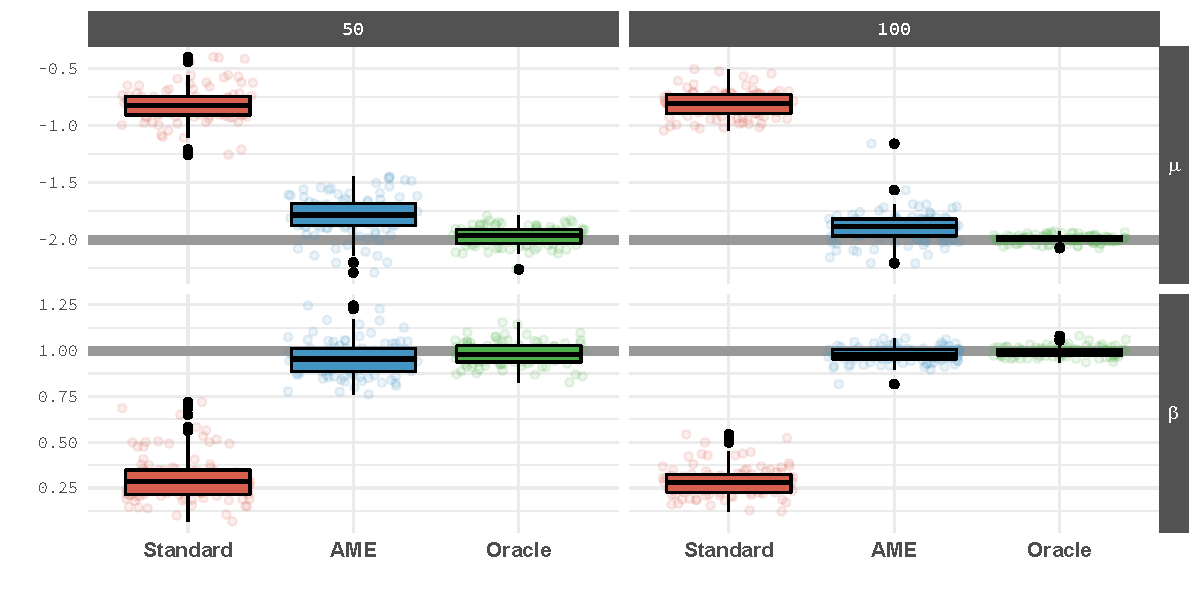
\includegraphics[width=1\textwidth]{ameSimBias_all_asaProbit.pdf} \\
	\end{figure}

	\begin{figure}[ht]
		\centering
		\caption{Proportion of times the true value fell within the estimated 95\% confidence interval for the standard, AME, and oracle models from 1,000 simulations.}
		\label{fig:ameCalib_asa}
		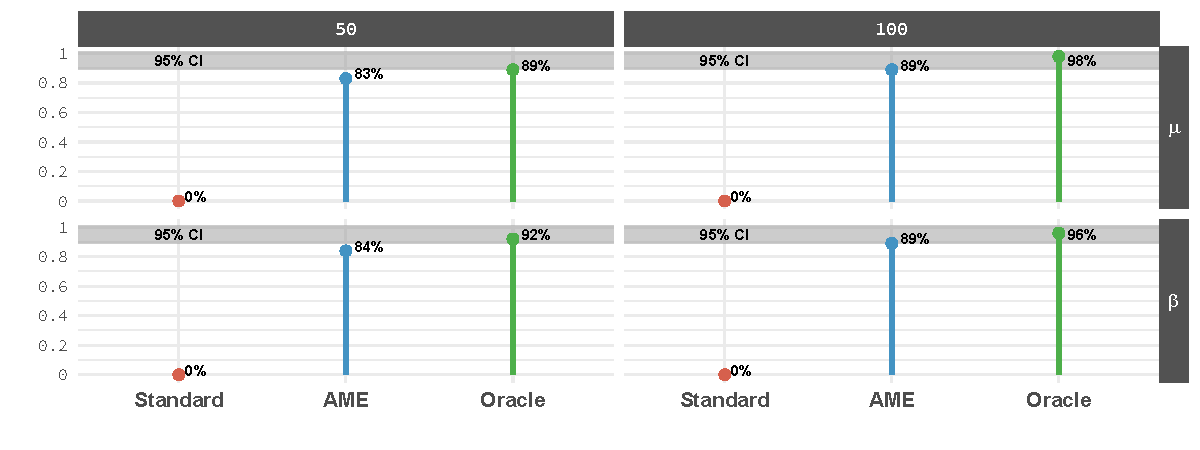
\includegraphics[width=1\textwidth]{ameSimCover_all_asaProbit.pdf} \\
	\end{figure}

	\end{itemize}
\end{enumerate}

\FloatBarrier
\clearpage

\section*{Reviewer 2}

\begin{enumerate}
	\item The additive and multiplicative effects (AME) model presented in the paper allows for a better treatment of first, second and third order dependencies in the data, and account for unobserved sources of bias in the data. The presentation of the AME estimator is clear, and the simulations provide clear evidence that the model outperforms naive OLS/GLM models fitted to the same data. The paper will be of great interest to the PSRM audience and is likely to have a strong impact on future research in international relations. I do, however, have a few suggestions for revisions that will hopefully strengthen the paper’s contributions.
	\begin{itemize}
		\item \textcolor{blue}{ \emph{
		We thank the reviewer for their comments and suggestions.
		}}
	\end{itemize}
	\item The paper shows that the AME model performs well in comparison to the “oracle” model where all sources of dependencies in the data are accounted for, which is reassuring. Yet this comparison feels incomplete. First, the naive model is clearly misspecified given the underlying data generating process. A large number of dependencies in international relations are linked to geography. What would happen if the dependencies were modeled using spatial econometric techniques?
	\begin{itemize}
		\item \textcolor{blue}{ \emph{
			The reviewer raises an important connection to the spatial literature. The types of geographic dependencies in international relations are generally monadic in nature -- civil war spreads from Rwanda to Uganda, or protest from Lebanon to Syria. With dyadic data, however, we cannot use the common geographic adjacency matrices used for normal spatial econometrics, because in dyadic data a W matrix would need to specify how dyad i,j relates to dyad k,l (for every i,j,k,l). In the simulation, we do not include a spatial lag model because this would require specifying a spatial dependence pattern (see Plumper and Neumayer 2010 for a more in-depth discuss on spatial lags). \textbf{CD}: I added this as a footnote on p.9. I moved this footnote around a LOT but I think it needs to live somewhere in the simulation. It felt awkward within the text.
			}}
%		CDMG: Flag for discussion. We brainstormed how to fit this into the simulation, but wouldn't simulating a W matrix be a bit arbitrary here?
%		Reference papers that have thought about what happens when we get the wrong W
%		general gist .. spatial models of dyadic dvs are great if we know how to characterize the diffusion amtrices, but the point of our approach is that we may not know how to actually characterize the ways in which actors are related to one another on some diffusion space.
%		reference franzesse et al mstar framework as a way to operationalize multiple pathways of diffusion in a spatial econometric approach
	\end{itemize}
	\item It would help if the author discussed in more depth the properties of the AME estimator in the presence of unobserved dependencies. One would imagine that the oracle model, where all the unobserved factors and dependencies are accounted for should always outperform a parametric or semi-parametric estimator. Relatedly, it also would help to have a more technical discussion of the properties of AME models, particularly in terms of the bias-variance trade off.
	\begin{itemize}
		\item \textcolor{blue}{ \emph{
		add example of case where omitted variable is correlated
		tech discussion bias-variance
		}}
	\end{itemize}
	\item The author could also underscore a related issue, which usually escapes empirical IR scholars: the importance of developing theories that account for the direct and indirect effects of interactions in a setting where the units are interconnected, and where the effects on one unit have the potential to impact other units in the system. A traditional approach is to throw as many observable variables as possible as controls, without much consideration on where they fit in the model. As the comparison of the AME and oracle models suggests, a careful modeling of spillovers and dependencies can result in better estimates of the underlying relationships.
	\begin{itemize}
		\item \textcolor{blue}{ \emph{
		We agree with this suggestion. We have now emphasized the importance of developing theory in our discussion of the AME and Oracle comparison (p. 13), as well as in the conclusion of our paper. We agree that innovations in dependence modeling can and should speak to theoretical advancements that, like our model, take into account the important relational and interdependent nature of political processes.
		}}
	\end{itemize}
	\item The paper emphasizes the importance of estimating the random effects for theory building and hypothesis test. A longer elaboration and illustration of this point would be very helpful.
	\begin{itemize}
		\item \textcolor{blue}{ \emph{
		We have added an additional interpretation of the random effects on pg. 19 in our discussion of Reiter and Stam. (``Specifically, we can see that countries such as Iraq, Israel, Egypt, and Iran are more likely to be involved in initiating or continuing conflict with other countries than the model would predict. Further, other countries such as Bhutan, Finland, and Turkmenistan are less likely to engage in conflict than the exogenous covariates in the model would suggest. In this case, the finding that countries in the middle east experience more conflict with other countries might lead one to more carefully examine the effects of geography on conflict initiation or to account for \citet{colgan:2010}'s theory that revolutionary petrostates are more aggressive.")
				}}
	\end{itemize}
	\item I would like to see a more detailed discussion of the setup and choices made for the Monte Carlo simulations. What type of network do the simulated data model? How does the network in the simulation relate to typical networks in IR studies, and to the ones in the replicated papers.
	\begin{itemize}
		\item \textcolor{blue}{ \emph{
		We've added additional discussion about how each of the variables in our simulation were generated. To make the model more applicable to the types of networks we study in IR we have provided a probit example. 
		}}
	\end{itemize}
	\item The criteria for choosing the studies for replication is unclear and needs a better justification. I would have liked to see a larger set of replications particularly in areas and topics where the data generating process, the dependencies among units varies, or the relationship between the units is hierarchical, cross-classified or multilevel.
	\begin{itemize}
		\item \textcolor{blue}{ \emph{
		We selected our cases based on a few criteria. We focus on studies that are explicitly about International Relations, were published since the year 2000, and were published in a top ranking general political science outlet (for consistency in editorial standards and reviews, we also decided to focus on one journal, the APSR). We hope that these three criteria ensure that our paper is readable and interpretable to an applied audience. In addition, we selected studies that could help illustrate different key components of the AME approach such as random effects (Reiter and Stam 2003), third-order dependencies (Weeks 2012), precision of fixed effects estimates (Gibler 2017).  While we agree with the reviewer that further replications would effectively demonstrate the benefits of the AME, we believe that they are beyond the scope of this paper at this time.
		}}
	\end{itemize}
	\item Given the importance of promoting the use of the AME method I would encourage the author to revise the tutorial presented in Appendix C to make it more accessible to a larger audience.
	\begin{itemize}
		\item \textcolor{blue}{ \emph{
		The reviewer raises a valid point. We have expanded our tutorial in Appendix C, particularly in giving more detail and concrete examples when it comes to formatting the data, which may represent the biggest hurdle for some users. We also...
		}}
	\end{itemize}
\end{enumerate}



\newpage\tiny
\end{document}\bye
